%%
%% Copyright 2019-2021 Elsevier Ltd
%%
%% This file is part of the 'CAS Bundle'.
%% --------------------------------------
%%
%% It may be distributed under the conditions of the LaTeX Project Public
%% License, either version 1.2 of this license or (at your option) any
%% later version.  The latest version of this license is in
%%    http://www.latex-project.org/lppl.txt
%% and version 1.2 or later is part of all distributions of LaTeX
%% version 1999/12/01 or later.
%%
%% The list of all files belonging to the 'CAS Bundle' is
%% given in the file `manifest.txt'.
%%
%% Template article for cas-dc documentclass for
%% double column output.

\documentclass[a4paper,fleqn]{cas-dc}

% If the frontmatter runs over more than one page
% use the longmktitle option.

%\documentclass[a4paper,fleqn,longmktitle]{cas-dc}

%\usepackage[numbers]{natbib}
%\usepackage[authoryear]{natbib}
\usepackage[authoryear,longnamesfirst]{natbib}
\usepackage{glossaries}\usepackage{multirow}
\usepackage{multirow}
\usepackage{subfig}
\usepackage[version=4]{mhchem}
\usepackage{hhline}
%%%Author macros
\def\tsc#1{\csdef{#1}{\textsc{\lowercase{#1}}\xspace}}
\tsc{WGM}
\tsc{QE}
%%%

\newcommand{\vect}[1]{\mathbf{#1}} % vectors and matrices

% Uncomment and use as if needed
%\newtheorem{theorem}{Theorem}
%\newtheorem{lemma}[theorem]{Lemma}
%\newdefinition{rmk}{Remark}
%\newproof{pf}{Proof}
%\newproof{pot}{Proof of Theorem \ref{thm}}

\begin{document}
\let\WriteBookmarks\relax
\def\floatpagepagefraction{1}
\def\textpagefraction{.001}

% Short title
\shorttitle{OpenMC transport independent depletion}

% Short author
\shortauthors{O. Yardas, P. Romano}

% Main title of the paper
\title [mode = title]{Extension of the OpenMC depletion module for indirect coupling with external transport solvers}

% Title footnote mark
% eg: \tnotemark[1]
%\tnotemark[<tnote number>]

% Title footnote 1.
% eg: \tnotetext[1]{Title footnote text}
%\tnotetext[<tnote number>]{<tnote text>}

% First author
%
% Options: Use if required
% eg: \author[1,3]{Author Name}[type=editor,
%       style=chinese,
%       auid=000,
%       bioid=1,
%       prefix=Sir,
%       orcid=0000-0000-0000-0000,
%       facebook=<facebook id>,
%       twitter=<twitter id>,
%       linkedin=<linkedin id>,
%       gplus=<gplus id>]

%\author[<aff no>]{<author name>}[<options>]
\author{Oleksandr Yardas}

% Corresponding author indication
\cormark[1]

% Footnote of the first author
\fnmark[1]

% Email id of the first author
\ead{oyardas2@illinois.edu}

% URL of the first author
%\ead[url]{<URL>}

% Credit authorship
% eg: \credit{Conceptualization of this study, Methodology, Software}
\credit{Methodology, Software, Validation, Visualization, Writing - original draft}

% Address/affiliation
\affiliation[1]{organization={Dept. of Nuclear, Plasma, and Radiological Engineering, University of Illinois Urbana-Champaign},
%            addressline={},
            city={Urbana},
%          citysep={}, % Uncomment if no comma needed between city and postcode
            postcode={61801},
            state={IL},
            country={USA}}

%\author[<aff no>]{<author name>}[<options>]
\author{Paul K. Romano}

% Footnote of the second author
\fnmark[2]

% Email id of the second author
\ead{promano@anl.gov}

% URL of the second author
%\ead[url]{}

% Credit authorship
\credit{Conceptualization, Methodology, Software, Funding acquisition, Writing - review and editing}

% Address/affiliation
\affiliation[2]{organization={Argonne National Laboratory},
            addressline={9700 S. Cass Ave},
            city={Lemont},
%          citysep={}, % Uncomment if no comma needed between city and postcode
            postcode={60439},
            state={IL},
            country={USA}}

% Corresponding author text
\cortext[1]{Corresponding author}

% Footnote text
\fntext[1]{}

% For a title note without a number/mark
%\nonumnote{}

% Here goes the abstract
\begin{abstract}
    We have implemented a new method for running depletion simulations in OpenMC
    that enables indirect coupling to any transport solver. The indirect
    coupling relies on using transport codes to calculate multigroup  microscopic cross
    sections. These microscopic cross sections are then used to calculate
    reaction rates, which are used to deplete materials using
    the existing algorithms in OpenMC's Python API.

    %% Rerun these cases with MG cases
    To validate this method, we ran simulations on a simple PWR pincell
    geometry. The new method allows depletion simulations to finish in a matter
    of seconds or minutes. The error for this new method scales with the size of
    the depletion timestep size. For ten 3-day timesteps, fission product errors
    are all under 3\%. Actinide errors range from 10-15\% for \ce{Am} and
    \ce{Cm}, 5-7\% for \ce{Pu} and \ce{Np}, and 2\% and less for \ce{U}. The
    large errors for certain actinides can be attributed to their small
    concentration and difficulty to produce accurately using one-group cross
    sections.

    Our results demonstrates the potential of this new method with moderate
    accuracy and extrodinary time savings for low and medium fidelity
    simulations.
\end{abstract}

% Use if graphical abstract is present
%\begin{graphicalabstract}
%\includegraphics{}
%\end{graphicalabstract}

% Research highlights
\begin{highlights}
\item A new method for running depletion calculations in OpenMC with indirect
    coupling to a transport solver
\item Moderate penalty in accuracy for some actinides for decreased calculation time
\item Low errors for fission products across the board
\end{highlights}

% Keywords
% Each keyword is seperated by \sep
\begin{keywords}
 Depletion \sep Coupling \sep OpenMC \sep Cross sections
\end{keywords}

\newacronym{crpg}{CRPG}{Computational Reactor Physics Group}
\newacronym{ornl}{ORNL}{Oak Ridge National Laboratory}
\newacronym{mit}{MIT}{Massachusets Institute of Technology}
\newacronym{csg}{CSG}{constructive solid geometry}
\newacronym{cfd}{CFD}{computational fluid dynamics}
\newacronym{cad}{CAD}{computer aided design}
\newacronym{dnp}{DNP}{delayed neutron precursor}
\newacronym{ghg}{GHG}{greenhouse gas}
\newacronym{gif}{GIF}{Generation IV International Forum}
\newacronym{msr}{MSR}{molten salt reactor}
\newacronym{msre}{MSRE}{Molten Salt Reactor Experiment}
\newacronym{msbr}{MSBR}{Molten Salt Breeder Reactor}
\newacronym{msfr}{MSFR}{Molten Sodium Fast Reactor}
\newacronym{nrc}{NRC}{Nuclear Regulatory Commission}
\newacronym{rnd}{R\&D}{research and development}
\newacronym{mns}{M\&S}{modeling and simulation}
\newacronym{ent}{E\&T}{education and training}
\newacronym{doene}{DOE-NE}{Department of Energy Office of Nuclear Energy}
\newacronym{cc}{CC}{closed code}
\newacronym{oss}{OSS}{open source software}
\newacronym{iaea}{IAEA}{International Atomic Energy Agency}
\newacronym{oncore}{ONCORE}{Open-source Nuclear COdes for REactor analysis}
\newacronym{snf}{SNF}{spent nuclear fuel}
\newacronym{sfr}{SFR}{sodium-cooled fast reactor}
\newacronym{doe}{DOE}{Department of Energy}
\newacronym{cram}{CRAM}{Chebyshev rational approximation method}

\maketitle

% Main text
\section{Introduction}\label{}
    %Modeling and simulation codes will play a critical role in licensing
    %advanced nuclear reactors. In preparation for advanced nuclear technology,
    %both the \Gls{doene} and the \Gls{nrc} identified several technical gaps in
    %current \Gls{mns} tools that are necessary for efficient and effective
    %license application reviews \citep{betzler_modeling_2019,
    %usnrc_nonlwr_2020-1}. Both \Gls{doene} and the \Gls{nrc} have specifically
    %identified depletion to be a key modeling feature for advanced nuclear
    %reactors.

    Recent projects seek to use state-of-the-art software tools in Monte Carlo
    transport and computational fluid dynamics coupled with heat transfer for
    simulating advanced reactors on exascale computing hardware to overcome the
    computational challenge of this task ~\citep{romano2021nse,merzari2023sc}.
    These methods are very computationally expensive, but deliver high
    confidence in their results. If any component in this tool chain could be
    simplified or sped up, it would greatly reduce the computational cost on and
    economic cost from these exascale machines.

    {\it Depletion} is the process by which the nuclide composition changes due
    to nuclear transmutation and decay reactions occurring in a material subject
    to irradiation. Depletion capabilities were recently added to OpenMC, an
    open source, community developed MC particle transport code
    \citep{romano_openmc_2015, romano_depletion_2021}. The depletion solver
    utilizes OpenMC's Python API to iteratively run a transport simulation,
    calculate the reaction rates, and update the material composition.
    In a reactor depletion calculation, there is a tight coupling between
    neutron transport and depletion because the change in material composition
    can result in changes to the spatial distribution of reaction rates.

    In the present work, we describe a new method for running depletion
    calculations without the need to iteratively run transport calculations by
    using precalculated microscopic cross sections and fluxes for each depletion
    step.  At most, only one transport calculation needs to be run to generate
    these cross sections and fluxes. If few materials are used, this effectively
    removes spatial effects of the changing material composition due to the
    static fluxes and cross sections. It is possible that spatial effects could
    be approximated by defining several materials for each fuel pin to capture
    radial and spatial effects, but this has not been tested.

    This limits the practical application of transport-independent depletion to
    domains where capturing spatial effects are a secondary concern. One
    such application is in global fuel-cycle analysis where we are more
    concerned with the overall change in material composition. Fuel cycle
    simulations typically model many different reactors simultaneously over
    long time periods. Performing transport-coupled depletions for each reactor
    at each timestep would be much more expensive than using
    transport-independent depletion. The capabilites described in this paper
    have been utilized in Cyclus \citep{huff_fundamental_2016} -- an open source
    fuel cycle simulator -- for coupling depletion to the fuel cycle
    simulaton \citep{bachmann_os_2024}. However, for other applications, the
    coupling between neutron transport and depletion is effectively one-way.
    This is often the case for experimental facilities with a neutron source
    where the source rate is high enough to cause activation of materials but
    not high enough to produce significant burnup of materials. Many proposed fusion
    energy facilities would fall into this category.  For such applications, there is
    no need to run a fully coupled simulation between neutron transport and
    depletion; instead, a neutron transport simulation corresponding to the
    beginning of irradiation can be carried out to determine reaction rates
    relative to the neutron source rate, and then the depletion calculation can
    be performed using the reaction rates scaled by any changes in the neutron
    source rate over time. For fusion systems, these calculations are often
    carried out with FISPACT-II~\citep{sublet2017nds}; See \citet{eade2020nf}
    for a recent example. The capabilities described in this paper have also
    been utilized for a recent study of shutdown dose rate in fusion
    systems~\citep{peterson2024nf}.

    This paper is organized as follows. In Section \ref{sec:methods}, we describe
    the methods and algorithms used to calculate reaction rates using the new
    depletion capabilities. In Section \ref{sec:results}, we describe our
    simulation and analyse the results. In Section \ref{sec:conclusion}, we
    summarize our results, and discuss some gaps in the current implementation
    of the new feature.



\section{Methodology}
    \label{sec:methods}
    Depletion is typically done in subregions that are small enough to have
    little spatial variation in the flux (and hence in the reaction rates). For
    example, in a full-core model, depletion regions may correspond to
    individual pincells, or even smaller sub-pin regions of radial rings and
    azimuthal segments. The general form of the equation governing depletion is
    %% The notation here matches what is in the OpenMC depletion paper from 2021
    \begin{equation}
      \label{eq:depletion}
      \begin{split}
        \frac{dN_i}{dt} = &\sum\limits_{j=1}^n \left[ \int_0^\infty 
        f_{j \rightarrow i}(E) \sigma_j (E, t) \phi(E,t) dE \;+ \lambda_{j\rightarrow i}
        \right] N_j(t) \\ &- \left [\int_0^\infty \sigma_i (E,t) \phi(E,t) dE \; +
        \sum\limits_{j=1}^n \lambda_{i\rightarrow j} \right ] N_i(t),
      \end{split}
    \end{equation}
    where
    \begin{equation*}
      \begin{split}
        N_i(t) &\equiv \text{density of nuclide $i$ at time $t$} \\
        \sigma_i(E,t) &\equiv \text{transmutation cross section for nuclide $i$ at energy $E$ and time $t$} \\
        \phi(E,t) &\equiv \text{neutron flux at energy $E$ and time $t$} \\
        f_{j \rightarrow i}(E) &\equiv \text{fraction of transmutation reactions in nuclide $j$ that produce nuclide $i$} \\
        \lambda_{j \rightarrow i} &\equiv \text{decay constant for decay modes in nuclide $j$ that produce nuclide $i$} \\
        n &\equiv \text{total number of nuclides.}
      \end{split}
    \end{equation*}
    The summations in Equation \ref{eq:depletion} are effectively over all
    nuclides excecpt $i$, as $f_{i \rightarrow i}(E)$ and $\lambda_{i \rightarrow i}$ must
    be zero by definition. Equation \ref{eq:depletion} can be condensed into a
    matrix-vector equation:
    \begin{equation}
      \label{eq:depletion-matrix-t}
      \frac{d\vect{n}}{dt} = \vect{A}(\vect{n},t)\vect{n}
    \end{equation}
    where
    \begin{equation}
      \vect{n} = \begin{pmatrix} N_1 \\ N_2 \\ \vdots \\ N_n \end{pmatrix}, \quad
    \end{equation}
    and $\vect{A}(\vect{n},t) \in \mathbb{R}^{n\times n}$ is the depletion
    matrix containing the decay and transmutation coefficients. The coefficients
    of $\vect{A}$ change with time and depend themselves on the nuclide
    composition vector $\vect{n}$, making this a nonlinear system of equations.
    OpenMC utilized the \Gls{cram} method to solve this system of equations
    \citep{romano_depletion_2021}. 
    
    We had two design goals for
    transport-independent depletion functionality:
    \begin{itemize}
        \item Enable use of OpenMC depletion capabilities using only the Python API.
        \item Enable depletion of materials directly given a multi-group flux
            for each material 
    \end{itemize}
    
    We created the \verb.IndependentOperator. and \verb.MicroXS. classes to
    achieve these design goals.    
    \subsection{MicroXS}
        \label{sub:microxs}
        The \verb.MicroXS. class contains cross-section data indexed by nuclide,
        reaction name, and energy group. It also contains methods to import and
        export \verb.MicroXS. objects from \verb,.csv, files. In principle, a
        user could create multi-group microscopic cross sections with a
        transport solver code, and then use the \verb.MicroXS.  class to read in
        the cross section data for use in depletion. However, this is
        unnecessary as the \verb.get_microxs_and_flux(). function runs an OpenMC
        $k$-eigenvalue calculation to create a \verb.MicroXS. object and
        multi-group flux profile for each user-specified domain.

        In the initial release of this feature in OpenMC v0.13.1, \verb.MicroXS.
        subclassed the Pandas \verb.DataFrame. class to store data and assumed a
        one-group structure. The v0.14.0 release removed the Pandas dependency
        and refactored \verb.MicroXS. class to store multi-group cross section
        data.

    \subsection{IndependentOperator}
        The \verb.Operator. class was refactored into a \verb.CoupledOperator.
        class maintaining the existing depletion cabability, and the
        transport-independent depletion machinery was implemented into a new
        class, \verb.IndependentOperator. which uses an instance of the
        \verb.MicroXS. class and corresponding fluxes for each depletion domain
        to calculate reaction rates for that domain using multi-group microscopic
        cross sections.

        Calculating reactions rates using multi-group cross sections is
        mathematically equivalent to tallying the reaction rates directly. In
        transport-coupled depletion calculation, the transmutation reaction
        rates $r_{ij}(t)$ are tallied directly as:
        \begin{equation}
            \label{eq:cont-rxn-rate}
            r_{ij}(t) = \left[\int_0^\infty \sigma_{ij}(E,t) \phi(E,t) dE \; \right]
            N_{i}(t)
        \end{equation}
        where $i$ and $j$ indicate the nuclide and reaction, respectively.
            To perform depletion using multi-group cross sections, the multi-group
        cross sections and fluxes are multiplied to get a per-source neutron
        reaction rate:
        \begin{equation}
            \label{eq:mg-rxn-rate}
            r_{ij}(t) = \left[\sum_{g} \sigma_{ij,g}(t) \phi_{g}(t) \right]
            N_{i}(t) 
        \end{equation}
        In the limit of infinitely small energy groups, Equation
        \ref{eq:mg-rxn-rate} is equivalent to \ref{eq:cont-rxn-rate}. In
        practice, to get a time-dependent microscopic cross section or flux, we
        must perform transport calculations (and in the case of time-varying
        microscopic cross sections, incorporate thermal feedbacks). Herein lies
        the primary assumption of transport-independent depletion: {\it
        microscopic cross sections and reactor fluxes are static}.

        %% THIS DOESN'T MATCH WITH OPENMCs COMMENTS
        Both the tallied and multi-group-calculated reaction rates have units of
        $\frac{\text{reactions}}{\text{src particle}}$. A normalization factor
        $f$ in $\frac{\text{src}}{\text{s}}$ is applied to obtain the more
        conventional unit of $\frac{\text{reactions}}{\text{s}}$:
        \begin{equation}
            R_{ij} = r_{ij} f
        \end{equation}
        This normalization factor is typcially related to the power of the
        reactor and energy released from fission (\verb.fission-q.
        normalization), or the external source strength (\verb.source-rate.
        normalization). \verb.IndependentOperator. may use either of these methods to normalize
        the reaction rates. normalizing the tally results, and computing
        reaction rates. While \verb.CoupledOperator. may use several methods to
        calculate fission yields, including using the Monte Carlo simulation to
        directly tally fission yields, \verb.IndependentOperator. relies on
        constant yield data included in the depletion chain file.

\section{Results}\label{sec:results}
    To validate this new feature, we performed a parameter scan study on a PWR
    pincell using a single depletion zone. Tables \ref{tab:mat-params},
    \ref{tab:fuel-comp}, \ref{tab:clad-comp}, and \ref{tab:water-comp} contain
    the material parameters of our model, and Table \ref{tab:geo-params}
    contains the geometric parameters.  We used the ENDF/B-VII.1 nuclear data
    library available at \url{openmc.org/official-data-libraries}. We used the
    ENDF/B-VII.1 depletion chain in the PWR spectrum available at
    \url{openmc.org/depletion-chains}.
    
    \begin{table}[<options>]
        \caption{Material Parameters}
        \label{tab:mat-params}
        \begin{tabular*}{\tblwidth}{@{}LLLL@{}}
            \toprule
             Item & Fuel & Cladding & Water \\ % Table header row
            \midrule
             Density [g/cc] & 10.4 & 6 & 1.0\\
             Volume [cc] & 0.1764$\pi$ & & \\
             S($\alpha$,$\beta$) &  & & \verb.c_H_in_H2O.\\
            \bottomrule
        \end{tabular*}
    \end{table}

    \begin{table}[<options>]
        \caption{Fuel Composition}
        \label{tab:fuel-comp}
        \begin{tabular*}{\tblwidth}{@{}LL@{}}
            \toprule
            Nuclide & Composition [at-\%] \\ % Table header row
            \midrule
             $^{15}$O & 0.000758 \\
             $^{16}$O & 1.999242 \\
             $^{234}$U & 0.000385 \\
             $^{235}$U & 0.043020 \\
             $^{236}$U & 0.000197 \\ 
             $^{238}$U & 0.956398 \\
             \bottomrule
        \end{tabular*}
    \end{table}

    \begin{table}[<options>]
        \caption{Cladding Composition}
        \label{tab:clad-comp}
        \begin{tabular*}{\tblwidth}{@{}LL@{}}
            \toprule
            Nuclide & Composition [at-\%] \\ % Table header row
            \midrule
             $^{90}$Zr & 0.5145 \\
             $^{91}$Zr & 0.1122 \\
             $^{92}$Zr & 0.1715 \\
             $^{94}$Zr & 0.1738 \\
             $^{96}$Zr & 0.028 \\ 
             \bottomrule
        \end{tabular*}
    \end{table}

    \begin{table}[<options>]
        \caption{Water Composition}
        \label{tab:water-comp}
        \begin{tabular*}{\tblwidth}{@{}LL@{}}
            \toprule
            Nuclide & Composition [at-\%] \\ % Table header row
            \midrule
             $^{1}$H & 1.999689\\
             $^{2}$H & 0.000311 \\
             $^{15}$O & 0.999621 \\
             $^{16}$O & 0.000379 \\
             \bottomrule
        \end{tabular*}
    \end{table}

    \begin{table}[<options>]
        \caption{Geometric Parameters}\label{tab:geo-params}
        \begin{tabular*}{\tblwidth}{@{}LLLL@{}}
            \toprule
            Fuel Radius & Clad Radius & Water Bounding Box dimensions\\
            \midrule
            0.42 & 0.45 &  1.24 $\times$ 1.24\\
            \bottomrule
        \end{tabular*}
    \end{table}
    We used time step size and depletion timestepper as our parameters to vary.
    Table \ref{tab:timestep-shorthands} shows the different time step sizes we
    used and their shorthand terminology. All simulations ran for 10 depletion
    steps.
    \begin{table}[<options>]
        \caption{}\label{tab:timestep-shorthands}
        \begin{tabular*}{\tblwidth}{@{}LL@{}}
            \toprule
            Time step sizes & Shorthand term \\ % Table header row
            \midrule
            360 seconds & Minutes\\
            4 hours & Hours\\
            3 days & Days\\
            30 days & Months\\
            \bottomrule
        \end{tabular*}
    \end{table}
    We used the \verb.PredictorIntegrator. time stepper, which is analagous to
    the Euler method. Predictor-corrector methods are not useful as neither the
    flux nor the cross sections are changing, only the timestep size.
    Preliminary testing with predictor-corrector methods showed that they
    actually {\it increased} the composition error magnitude compared to
    predictor corrector methods. We used \verb.fission-q. normalization for all
    cases with a linear power density of 174 W/cm.  For each parameter
    combination, we ran with three cases:
    \begin{enumerate}
        \item Transport-coupled depletion
        \item Transport-independent depletion
        \item Transport-independent depletion with microscopic cross sections
            updated after each depletion step (one-group only).
    \end{enumerate}

    For the first case, we used 25 inactive and 125 active batches, with $10^6$
    particles per batch. For transport independent depletion, we used three
    different group strucutres to test the effect on the accuracy: one group,
    CASMO-8, and CASMO-40.

    Note that the third case is significantly slower than transport-coupled
    depletion as the cross sections need to be reloaded after each depletion
    step. Due to the cross section discretization that occurs before peforming
    depletion, we do not expect the third case results to converge to the first
    case results in limit of infinite particles. We would expect the third case
    to converge in the limit of infinite particles and energy groups. The third
    case was only run for one-group transport-independent depletion. Unless
    otherwise specified, all results are using 3-day time steps and
    \verb.PredictorIntegrator. The general trend is that concentration errors
    are smaller for shorter depletion time steps, and larger for longer
    depletion time steps, however there are more complicated dynamics for this
    to be a reliable prediction for each nuclide concentration.

    % actinides error 
    \begin{figure}[h!tpb]
        \centering
        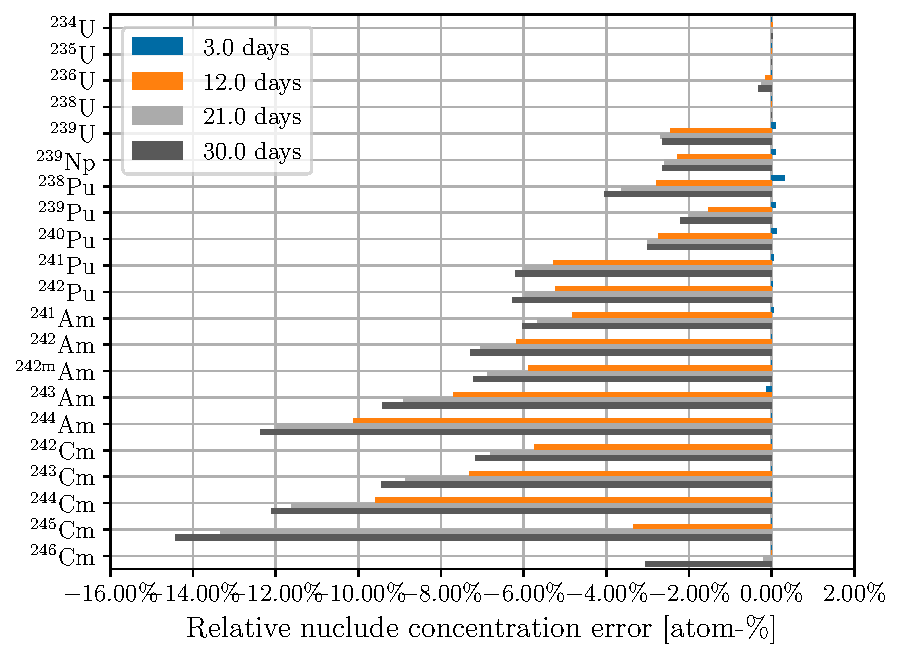
\includegraphics[width=\linewidth]{figs/actinides_constant_xs_predictor_fission_q_days.pdf}
        \caption[]{Relative error of predicted actinide concentrations using
        constant cross sections and 3-day time steps}
        \label{fig:actinides-error-constant-xs-days}
    \end{figure}

    \begin{figure}[h!tpb]
        \centering
        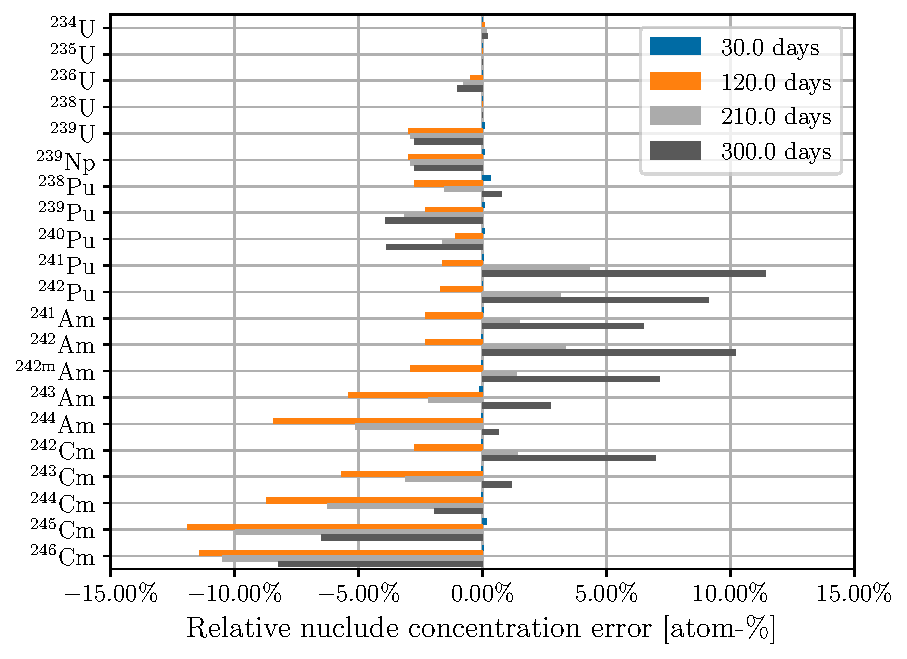
\includegraphics[width=\linewidth]{figs/actinides_constant_xs_predictor_fission_q_months.pdf}
        \caption{Relative error of predicted actinide error using
        constant cross sections and 30-day time steps}
        \label{fig:actinides-error-constant-xs-months}
    \end{figure}

    Figures \ref{fig:actinides-error-constant-xs-days} and
    \ref{fig:actinides-error-updating-xs-days} show the relative error for
    actinides using constant cross sections and updating cross sections,
    respectively, using 3-day time steps. Figures
    \ref{fig:actinides-error-constant-xs-months} and
    \ref{fig:actinides-error-updating-xs-months} show the same respective
    quantities for 30-day time steps. As expected, updating the cross sections
    at each depletion step results in very low errors, on the order of a
    fraction of a percent. The error trend for constant cross sections depends
    both on the cross section and time step size. For example, constant cross
    sections using a 3-day time step underpredicts the \ce{^{241}Pu}
    concentration, but at longer time steps overpredicts the concentration. The
    overprediction is due due to overcalculating the rate of ($n,\gamma$)
    reactions that occur on \ce{^{240}Pu}. Figure \ref{fig:pu240-n-gamma-months}
    shows this.

    \begin{figure}[htpb]
        \centering
        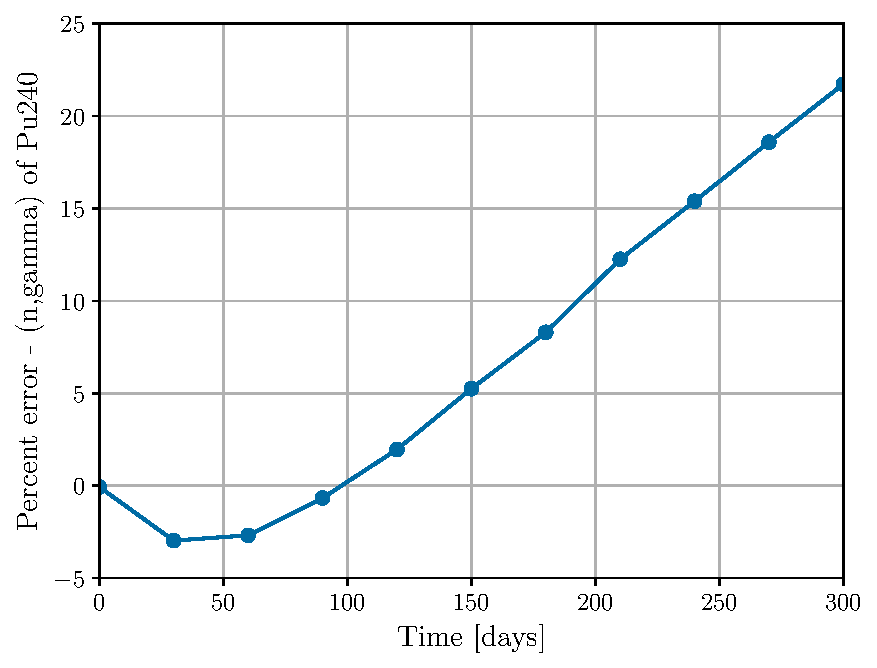
\includegraphics[width=\linewidth]{figs/pu240-n-gamma-months.pdf}
        \caption{Relative error of predicted \ce{^{240}Pu} ($n,\gamma$)
            reactions using constant cross sections and 30-day time steps}
        \label{fig:pu240-n-gamma-months}
    \end{figure}

    The error timeseries of \ce{^{241}Pu} is reproduced in daughter nuclides
    that are related to the amount of \ce{^{241}Pu}, such as isotopes of \ce{Cm}
    and \ce{Am}. We observe a general trend that the less important or abundant
    nuclides have higher concentration error relative to transport-coupled
    depletion. The less abundant actinides have increased sensitivity to over or
    underestimations of production.  The more important nuclides (\ce{U},
    \ce{^{239}Np}, \ce{^{239}Pu}, \ce{^{240}Pu}) tend to have low concentration
    errors, (5\% or less), whereas the less important actinides (Am, Cm,
    \ce{^{241}Pu}, \ce{^{242}Pu}) tend to have very high (more than 10\%)
    depending on the nuclide of interest.

    \begin{figure}[htpb]
        \centering
        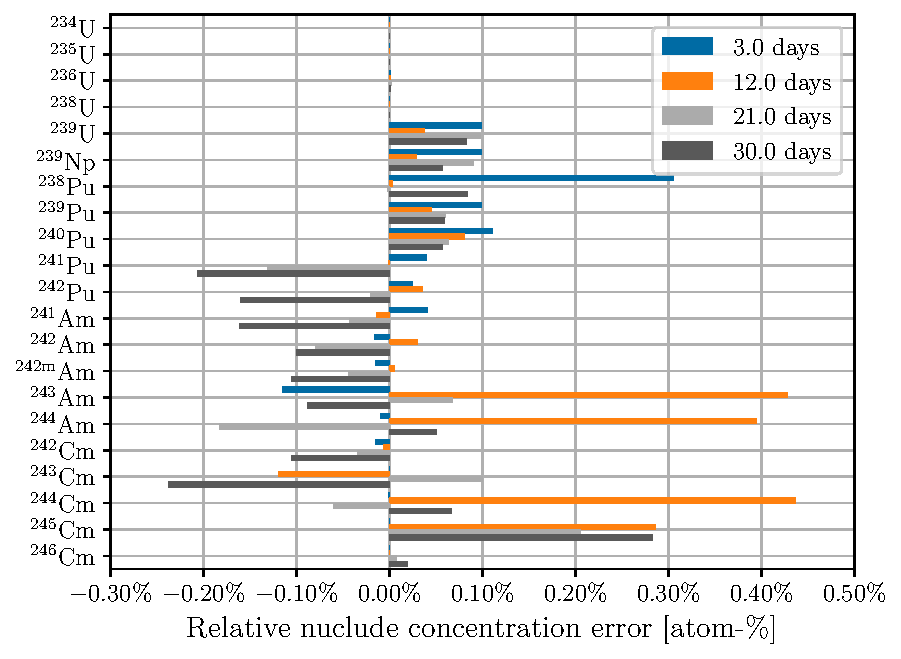
\includegraphics[width=\linewidth]{figs/actinides_updating_xs_predictor_fission_q_days.pdf}
        \caption{Relative error of predicted actinide error using
        updating cross sections and 3-day time steps}
        \label{fig:actinides-error-updating-xs-days}
    \end{figure}

    \begin{figure}[htpb]
        \centering
        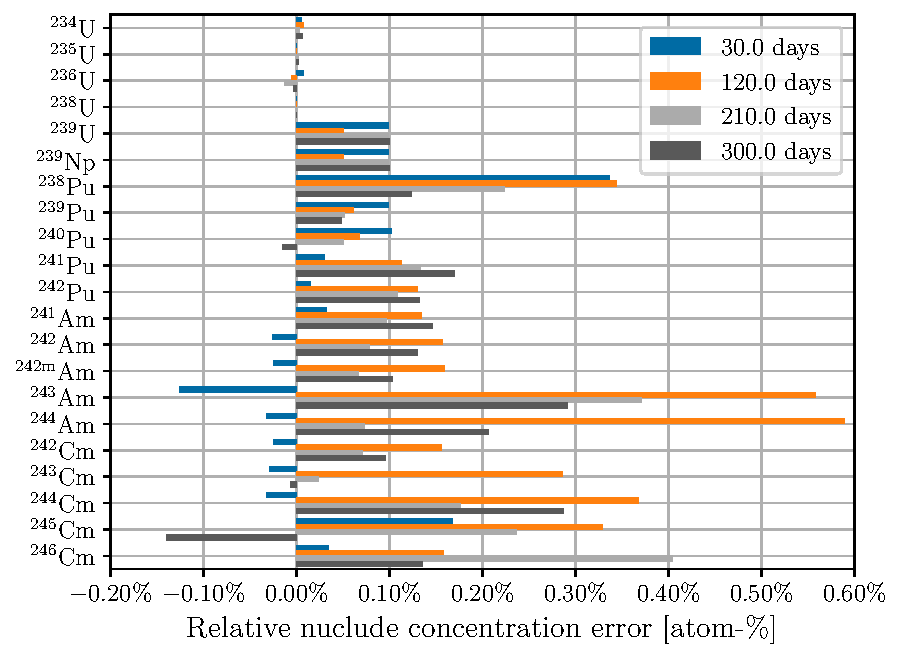
\includegraphics[width=\linewidth]{figs/actinides_updating_xs_predictor_fission_q_months.pdf}
        \caption{Relative error of predicted actinide error using
        updating cross sections and 30-day time steps}
        \label{fig:actinides-error-updating-xs-months}
    \end{figure}


    Figures \ref{fig:fp-error-constant-xs-days} and
    \ref{fig:fp-error-updating-xs-days} show the relative error for fission
    products using constant cross sections and updating cross sections,
    respectively, using 3-day time steps. Figures
    \ref{fig:fp-error-constant-xs-months} and
    \ref{fig:fp-error-updating-xs-months} show the same respective quantities
    for 30-day time steps. Similar to the actinides, updating the cross sections
    at each time step results in very low nuclide composition errors. There is a
    notably lower error across the board for many of these fission products
    compared to the actinides. This can simply be explained by the low
    composition error of \ce{^{235}U}. The majority of the fissile material in
    the fuel is \ce{^{235}U}, so the composition error of fission products
    produced should also be relatively low. Other actinides with higher
    composition errors are orders of magnitude less abundant in the fuel, so
    their effect on fission product composition error is proportionaly small.

    Composition errors for low-abundance nuclides using 30-day timesteps follow
    an interesting trend where there is an initial large negative error
    composition error that becomes more positive over time. This behavior is due
    to overestimation of nuclide production due to static cross sections and
    fluxes.

% fission products error
    \begin{figure}[h!tpb]
        \centering
        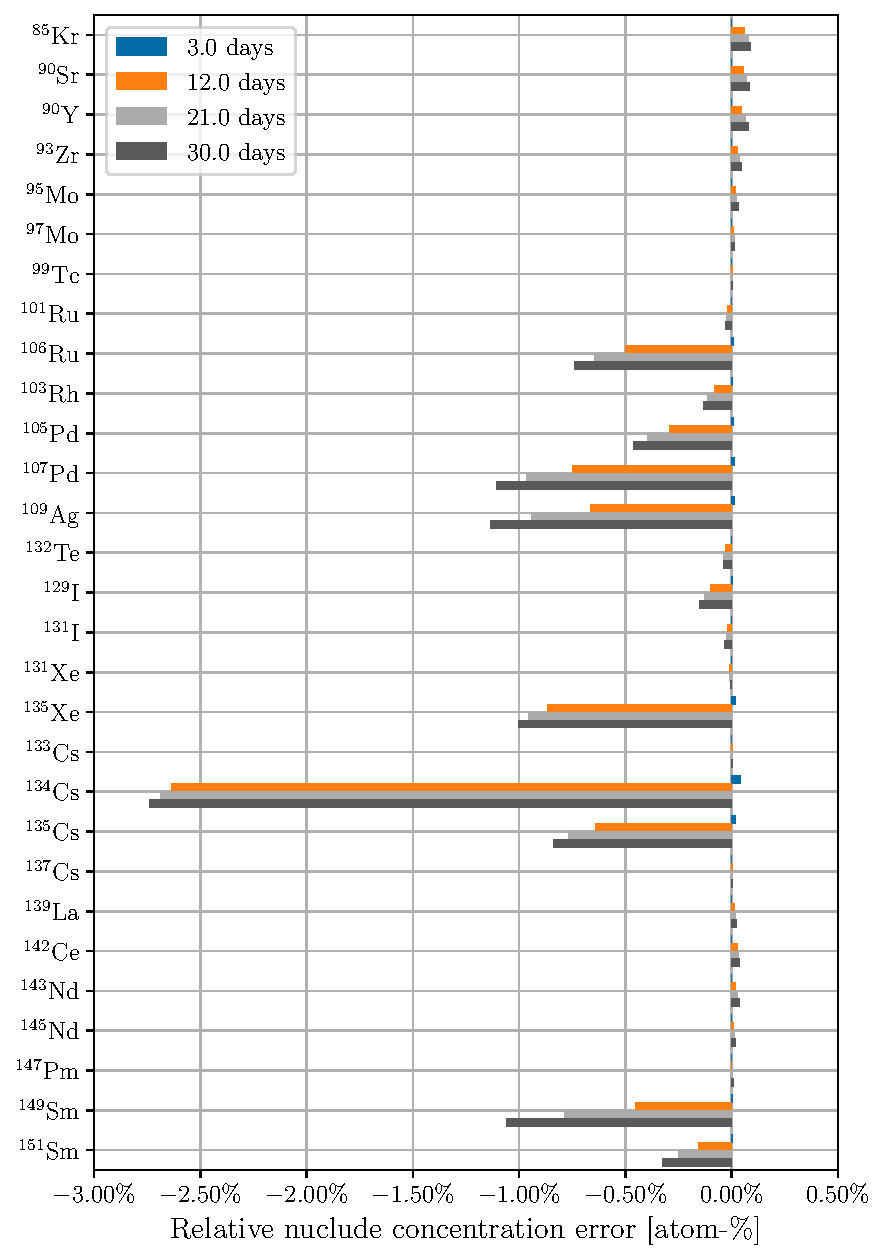
\includegraphics[width=\linewidth]{figs/fission_products_constant_xs_predictor_fission_q_days.pdf}
        \caption{Relative error of predicted fission product concentrations
        using constant cross sections and 3-day time steps}
        \label{fig:fp-error-constant-xs-days}
    \end{figure}

    \begin{figure}[htpb]
        \centering
        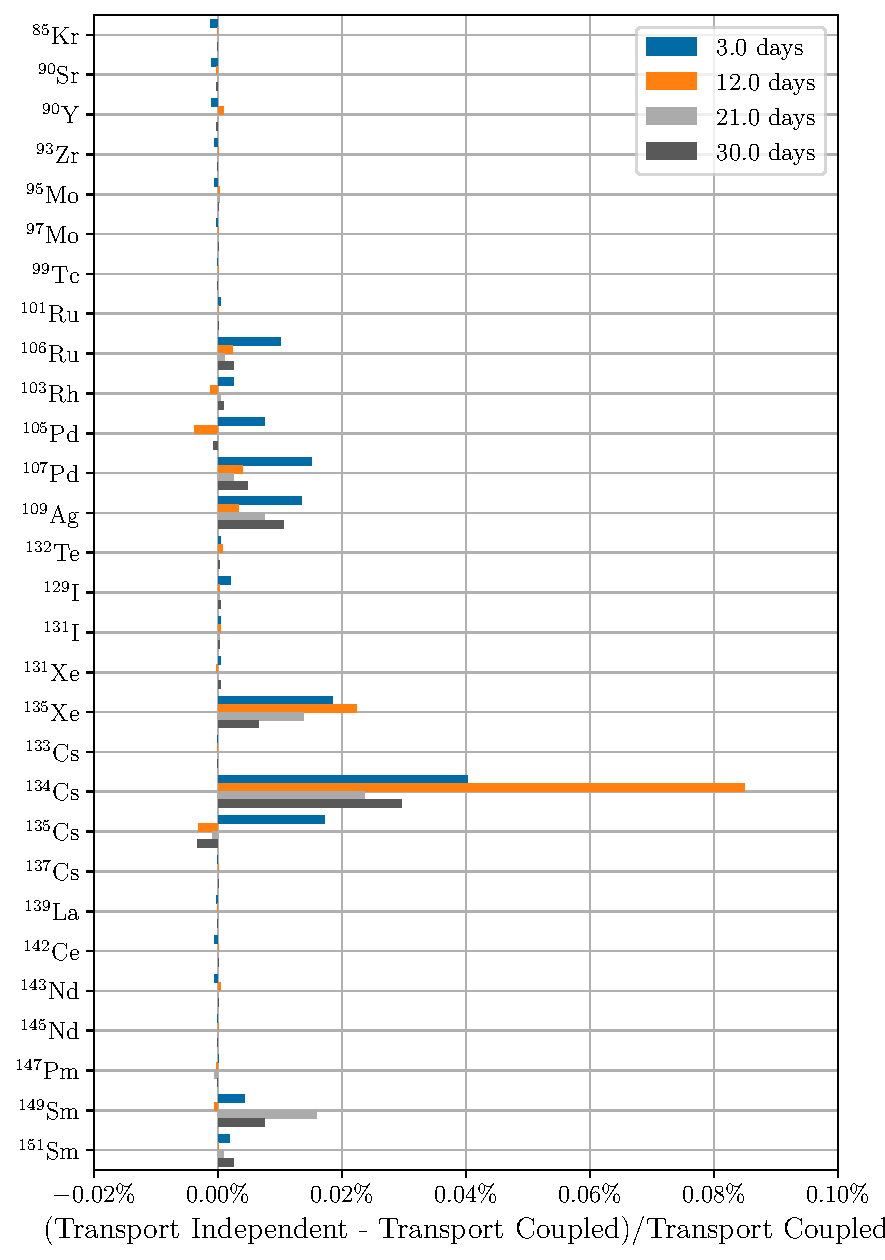
\includegraphics[width=\linewidth]{figs/fission_products_updating_xs_predictor_fission_q_days.pdf}
        \caption{Relative error of predicted fission product error using
        updating cross sections and 3-day timesteps}
        \label{fig:fp-error-updating-xs-days}
    \end{figure}
 
    \begin{figure}[htpb]
        \centering
        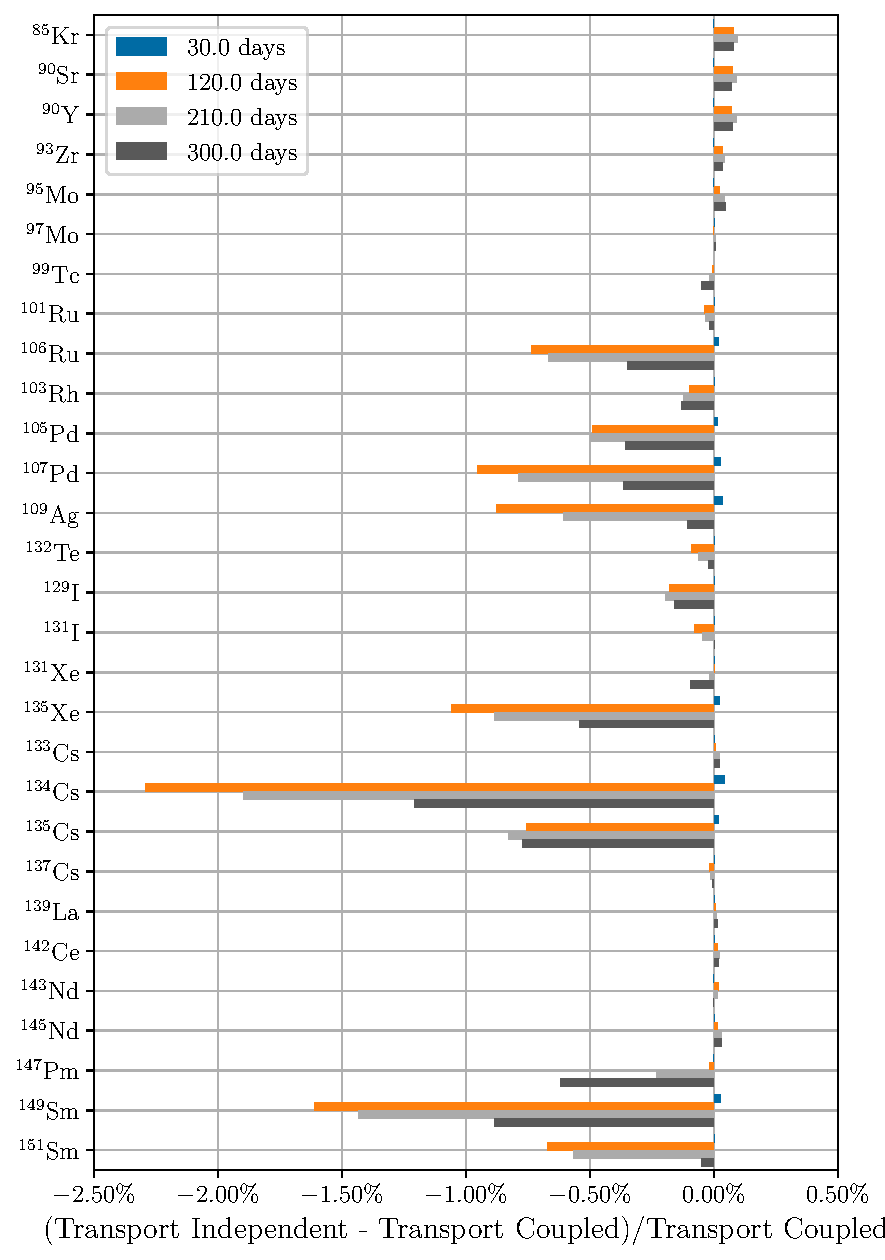
\includegraphics[width=\linewidth]{figs/fission_products_constant_xs_predictor_fission_q_months.pdf}
        \caption{Relative error of predicted fission product error using
        constant cross sections and 30-day time steps}
        \label{fig:fp-error-constant-xs-months}
    \end{figure}

    \begin{figure}[htpb]
        \centering
        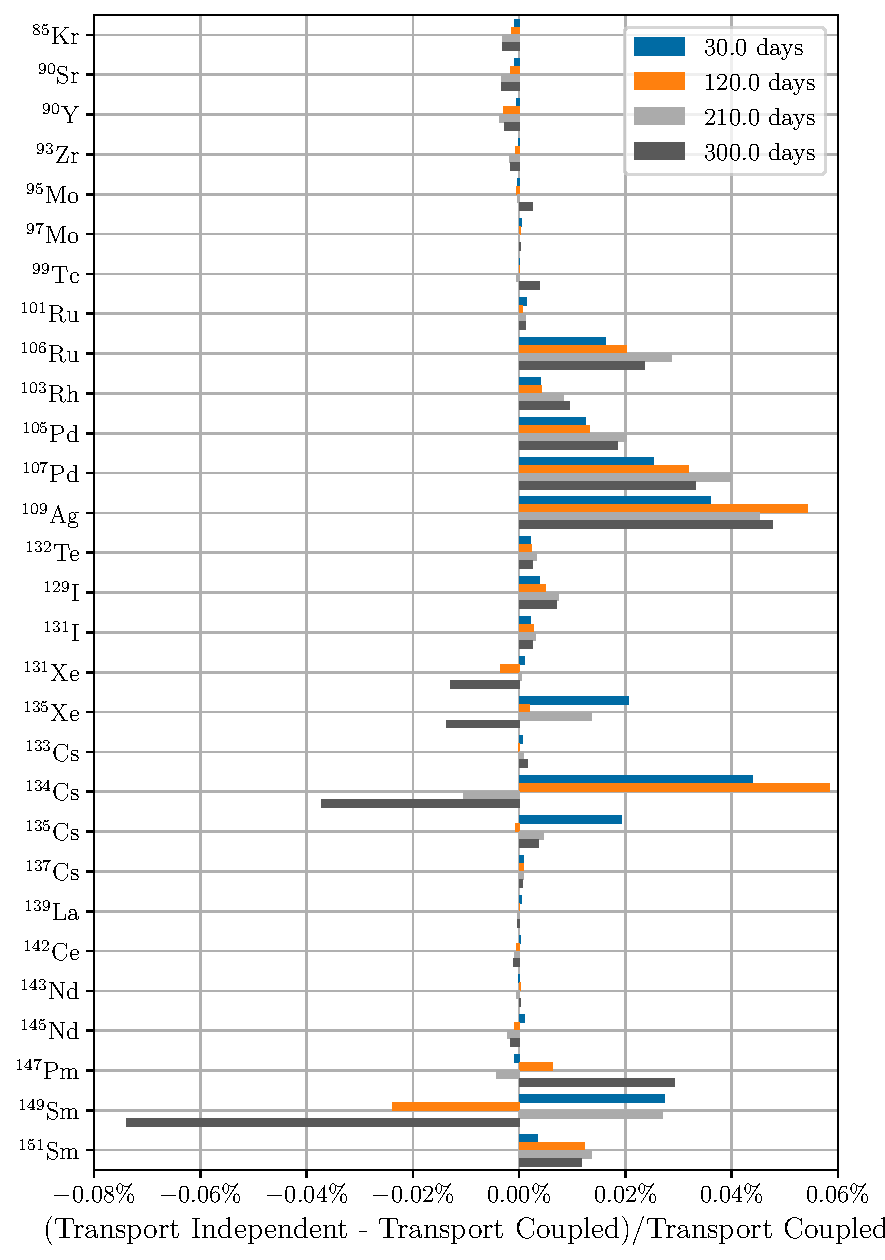
\includegraphics[width=\linewidth]{figs/fission_products_updating_xs_predictor_fission_q_months.pdf}
        \caption{Relative error of predicted fission product error using
        updating cross sections and 30-day time steps}
        \label{fig:fp-error-updating-xs-months}
    \end{figure}

    Repeating this analysis for both the CASMO-8 and CASMO-40 multi-group
    strucutres did not yield significant decreases in error for
    transport-independent depletion over the one-group case.  Figures
    \ref{fig:actinides-error-casmo8-xs-days} and
    \ref{fig:actinides-error-casmo40-xs-days} show the relative error for
    fission products using the CASMO-8 and CASMO-40 group structures,
    respectively, using 3-day time steps. Figures
    \ref{fig:actinides-error-casmo8-xs-months} and
    \ref{fig:actinides-error-casmo40-xs-months} show the same respective
    quantities for 30-day time steps.  It is possible in more complication
    models, like full reactor depletion, that the multi-group strucutre will
    become more important. 

    \begin{figure}[h!tpb]
        \centering
        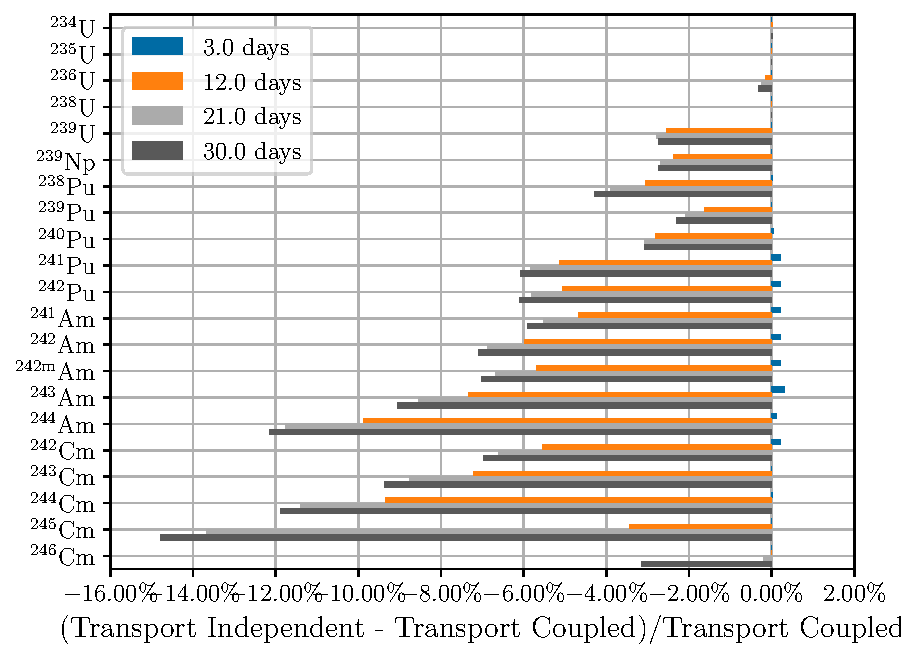
\includegraphics[width=\linewidth]{figs/actinides_casmo8_constant_xs_predictor_fission_q_days.pdf}
        \caption[]{Relative error of predicted actinide concentrations using
        CASMO-8 group structure and 3-day time steps}
        \label{fig:actinides-error-casmo8-xs-days}
    \end{figure}

    \begin{figure}[h!tpb]
        \centering
        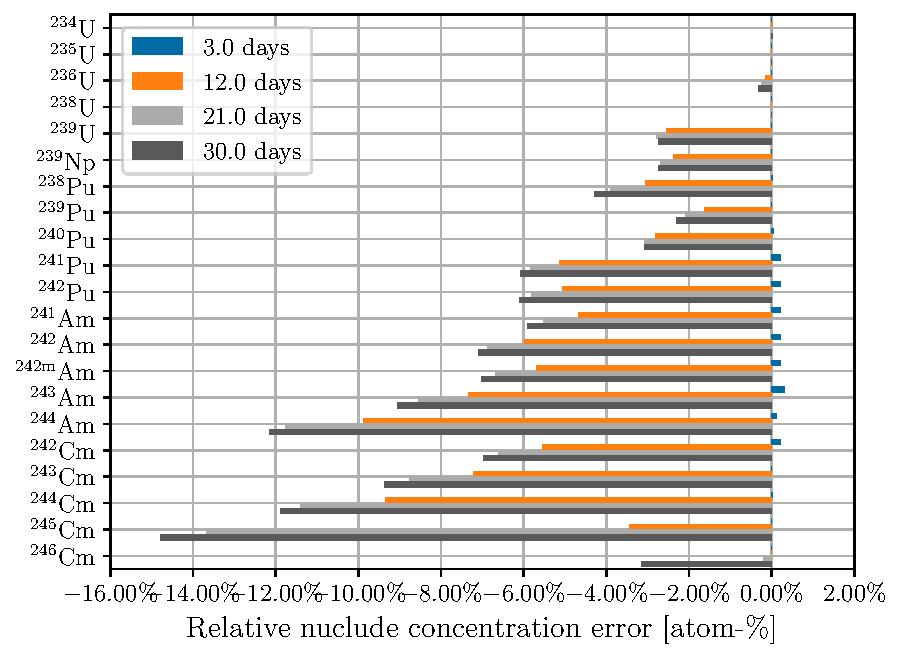
\includegraphics[width=\linewidth]{figs/actinides_casmo40_constant_xs_predictor_fission_q_days.pdf}
        \caption{Relative error of predicted actinide error using
        CASMO-40 group structure and 3-day time steps}
        \label{fig:actinides-error-casmo40-xs-days}
    \end{figure}

    \begin{figure}[h!tpb]
        \centering
        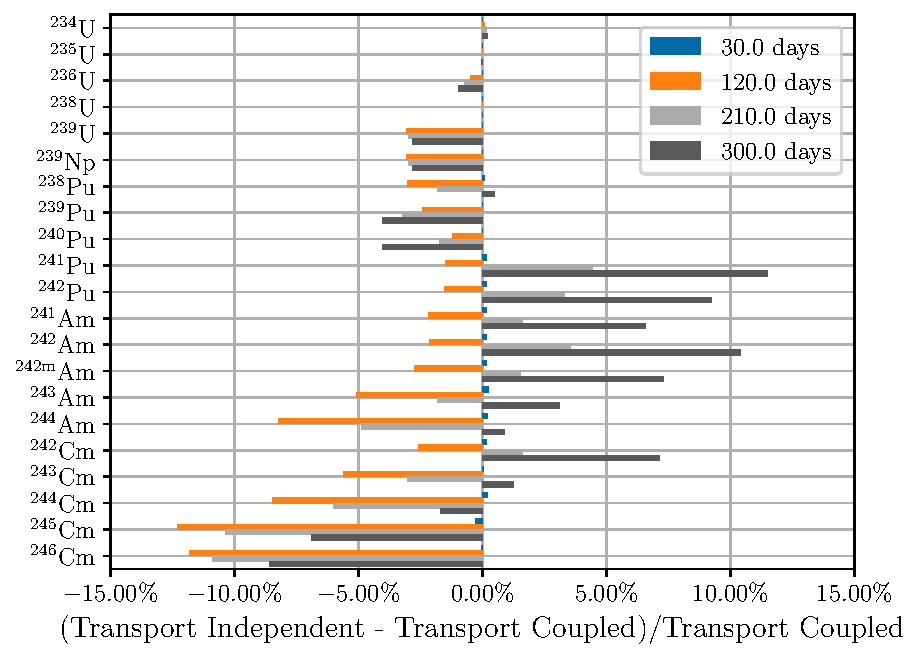
\includegraphics[width=\linewidth]{figs/actinides_casmo8_constant_xs_predictor_fission_q_months.pdf}
        \caption[]{Relative error of predicted actinide concentrations using
        CASMO-8 group structure and 30-day time steps}
        \label{fig:actinides-error-casmo8-xs-months}
    \end{figure}

    \begin{figure}[h!tpb]
        \centering
        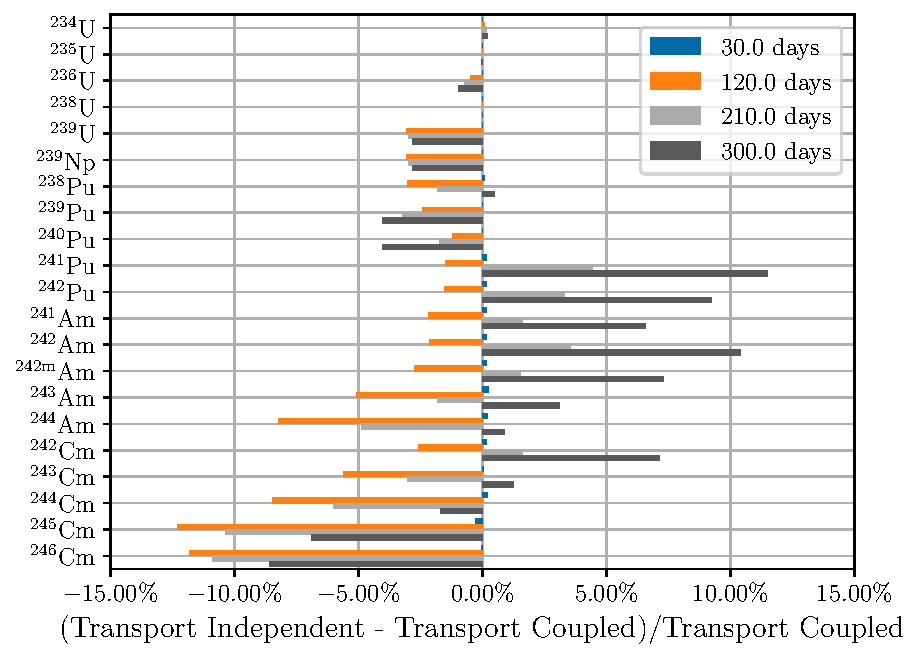
\includegraphics[width=\linewidth]{figs/actinides_casmo40_constant_xs_predictor_fission_q_months.pdf}
        \caption{Relative error of predicted actinide error using
        CASMO-40 group structure and 30-day time steps}
        \label{fig:actinides-error-casmo40-xs-months}
    \end{figure}


    The time savings when using \verb.IndependentOperator. are immense. Whereas
    the transport-coupled simulations each took several hours to complete, the
    transport-independent simulations took seconds to minutes to complete!

\section{Conclusions}\label{sec:conclusion}
    In this paper, we introduced transport-independent depletion in OpenMC. This
    method utilized pre-computed multi-group cross sections and fluxes to
    calculate reaction rates for a depletion calculation. The new method is
    siginifcantly faster than running a transport-coupled depletion simulation,
    albiet with a penalty to accuracy. Better accuracy will be obtained for
    models where the neutron flux spectrum will be constant, i.e. in
    fusion systems, low power fission reactors, and .
         
    This study focused exclusively on nuclide compositions. No capability exists
    in \verb.IndependentOperator. to monitor criticality as the fuel depletes. A
    good starting point may be in implementing a method similar to the method to
    estimate $k_{\infty}$ used in \cite{LOVECKY2014333}, wherein
    \begin{equation}
        k_{\infty} = \frac{\sum_{i} \sum_{j} N_{i} \nu_{j}
        \sigma_{i}^{j}}{\sum_{i}\sum_{j} N_{i} \sigma_{i}^{j}}  
    \end{equation}
    where $j$ indicates the type of reaction, and $\nu_{j}$ is the neutron
    multipliation of reaction $j$, defined as
    \begin{equation}
        \nu_j = \begin{cases}
            0 & j=\text{ absorption reaction}\\
            x & j=(n,xn)\\
            \bar{\nu} & j=\text{fission}
        \end{cases}
    \end{equation}
    In OpenMC, $(n,xn)$ reactions are not used to calculate $k_\text{eff}$ (and
    by extension $k_{\infty}$). In this case, $\nu_{x} = 0$ in the numerator for
    all $x$, and we would use an `effective' aborption cross section
    $\overline{\sigma}_{a} = \sigma_{a} - \sigma_{(n,2n)} - 2\sigma_{(n,3n)} -
    3\sigma_{(n,4n)}$. 

    The geometry used in this study was a simple PWR pincell. We did not find
    significant difference in error between one-group, 8-group, and 40-group
    transport-independent depletion. It is possible that this distinction
    becomes more important for complex geometries with distinct depletion zones.


% Numbered list
% Use the style of numbering in square brackets.
% If nothing is used, default style will be taken.
%\begin{enumerate}[a)]
%\item
%\item
%\item
%\end{enumerate}

% Unnumbered list
%\begin{itemize}
%\item
%\item
%\item
%\end{itemize}

% Description list
%\begin{description}
%\item[]
%\item[]
%\item[]
%\end{description}

% Figure
%\begin{figure}[<options>]
%	\centering
%		\includegraphics[<options>]{}
%	  \caption{}\label{fig1}
%\end{figure}


%\begin{table}[<options>]
%\caption{}\label{tbl1}
%\begin{tabular*}{\tblwidth}{@{}LL@{}}
%\toprule
%  &  \\ % Table header row
%\midrule
% & \\
% & \\
% & \\
% & \\
%\bottomrule
%\end{tabular*}
%\end{table}

% Uncomment and use as the case may be
%\begin{theorem}
%\end{theorem}

% Uncomment and use as the case may be
%\begin{lemma}
%\end{lemma}

%% The Appendices part is started with the command \appendix;
%% appendix sections are then done as normal sections
%% \appendix

% To print the credit authorship contribution details
\printcredits

%% Loading bibliography style file
%\bibliographystyle{model1-num-names}
\bibliographystyle{cas-model2-names}

% Loading bibliography database
\bibliography{bibliography}

% Biography
%\bio{}
% Here goes the biography details.
%\endbio

%\bio{pic1}
% Here goes the biography details.
%\endbio

\end{document}

